\documentclass[11pt]{article}
\usepackage{tikz}
\usepackage{amsmath}
\usepackage{mathtools}

%\usepackage{xfrac}
%\usepackage{hyperref}
%\usepackage[export]{adjustbox}
\def\checkmark{\tikz\fill[scale=0.4](0,.35) -- (.25,0) -- (1,.7) -- (.25,.15) -- cycle;} 
\usepackage{proj} 	% pull in style header
\usepackage{array}
\usepackage{sectsty}
\usepackage{soul}
\usepackage{float}
\restylefloat{table}

\lhead{ECE582: Formal Verification}


%----------------------------------------------------------------------------------------
%	TITLE SECTION
%----------------------------------------------------------------------------------------


\newcommand{\horrule}[1]{\rule{\linewidth}{#1}} % Create horizontal rule command with 1 argument of height

\title{	
\normalfont \normalsize 
\textsc{\LARGE Portland State University}\\[1.5cm] % Name of your university/college
\textsc{\Large Project 2}\\[0.5cm] % Major heading such as course name
\textsc{\large ECE582}\\[0.5cm] % Minor heading such as course title
%\textsc{Portland State University} \\ [25pt] % Your university, school and/or department name(s)
\horrule{1.2pt} \\[0.4cm] % Thin top horizontal rule
\huge Model Checking by NuSMV \\ % The assignment title
\horrule{1.2pt} \\[0.5cm] % Thick bottom horizontal rule
}

%----------------------------------------------------------------------------------------
%	AUTHOR SECTION
%----------------------------------------------------------------------------------------


\begin{document}\raggedright
\author{Erik Rhodes \and Jordan Fluth} % Your name
\maketitle % Print the title
\thispagestyle{empty}
\cfoot{\textit{Page \thepage { of} \pageref{LastPage}}}
\lhead{ECE582}
\chead{Project 2}
\rhead{Erik Rhodes \& Jordan Fluth}


\begin{figure}[h]\centering

\includegraphics[height=0.65\textwidth]{images/sat_intro.jpg}
	%\caption{Gameplay Block Diagram}
		\label{LED}
	\end{figure}
	
\newpage

% -------------------------PROJECT DELIVERABLES
%Part 1:
%Make circuit with 9 gates
%Draw circuit
%Make another identical copy C2. Prove C1=C2 by a Sat solver automatically.
%Download a SAT solver for satisfiability
%
%Part 2:
%Replace one gate with a different one
%Prove/disprove C1=C3 by a SAT solver automatically
%
%For the report, describe:
%Method to check equivalence by a SAT solver
%All CNF forms used in the proof
%All formulas and figures should be typed and drawn in software
%Detailed discussion of our derivation and solution



\section{Introduction} 
Talk about model checking


%\begin{figure}[h]\centering
%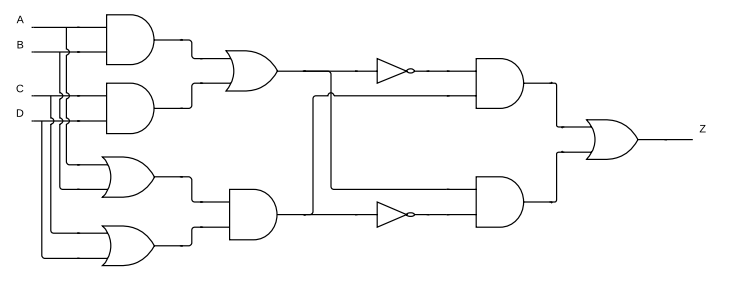
\includegraphics[height=0.45\textwidth]{images/c1.PNG}
%	\caption{Original Circuit}
%		\label{c1}
%	\end{figure}


%Symbols \And \wedge \vee \neg \to \gets \iff


\section{Combinational Lock}
	\subsection{NuSMV}
	\subsection{Added properties}
	\subsection{Results}

%\begin{figure}[h!]\centering
%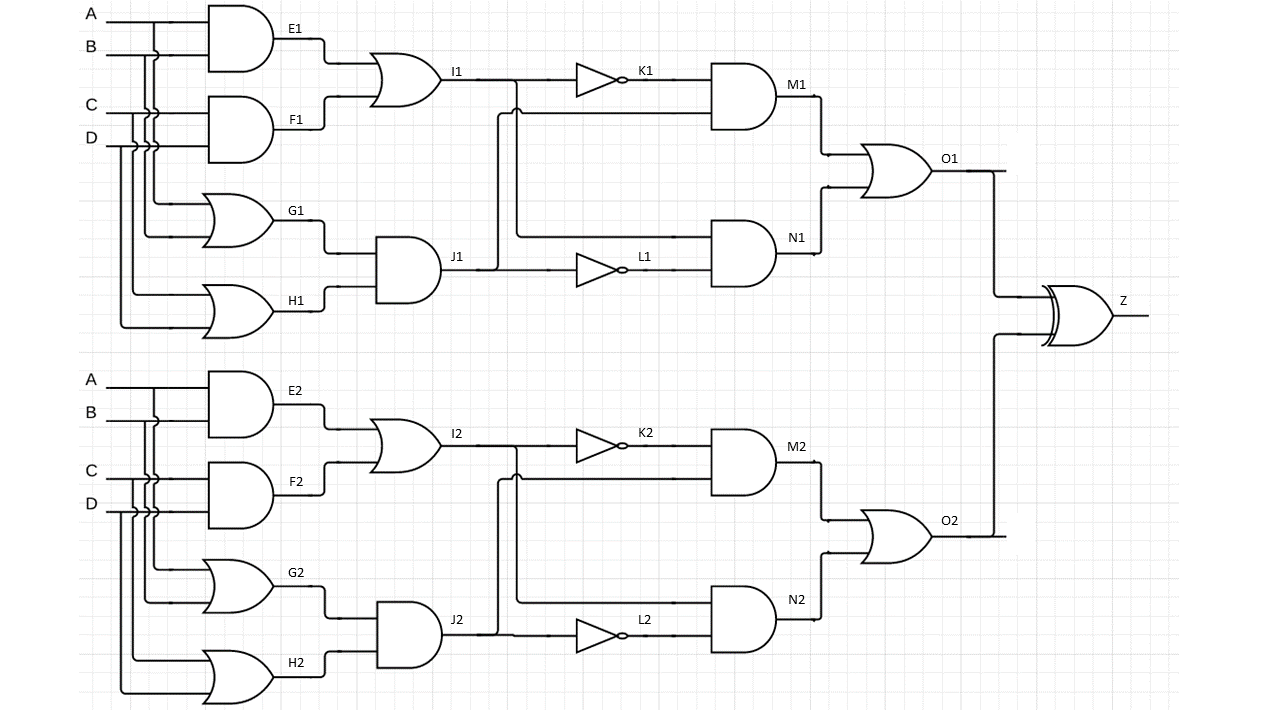
\includegraphics[height=0.55\textwidth]{images/c1c2.PNG}
%	\caption{Miter Circuit of C1 and C2}
%		\label{c2}
%	\end{figure}

\section{Kripke Structures} 

\subsection{Figure 1}
	\subsection{NuSMV}
	\subsection{Added properties}
	\subsection{Results}
\subsection{Figure 2}
	\subsection{NuSMV}
	\subsection{Added properties}
	\subsection{Results}

%\vspace{12pt}
%
%\begin{figure}[h]\centering
%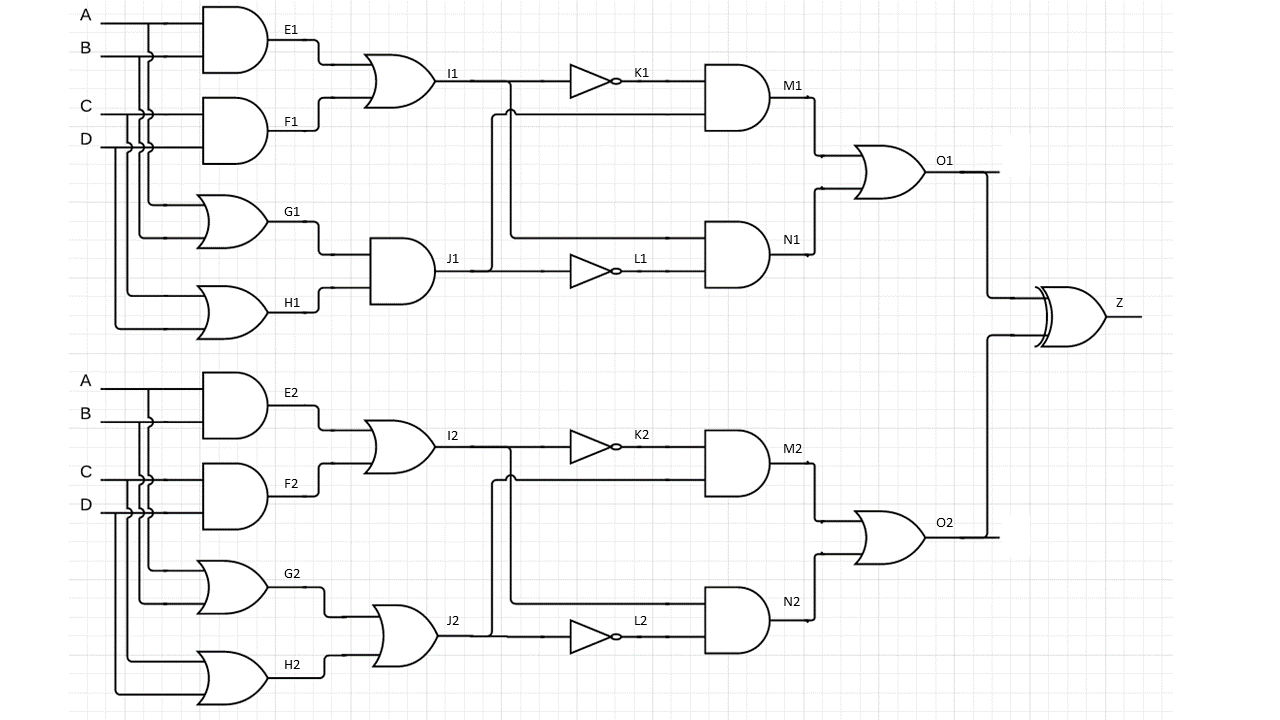
\includegraphics[height=0.5\textwidth]{images/c1c3.PNG}
%	\caption{Miter Circuit of C1 and C3}
%		\label{c3}
%	\end{figure}

\section{Equivalence Checking} 
\subsection{NuSMV}
\subsection{Results}
System Diameter.
Reachable states
Check AG(output=0)

%  
%\section{Results}
%Do we need to show any output from boolsat.com?
\end{document}